\section{Concepción y Diseño}\label{section:design}

\begin{figure}
    \centering
    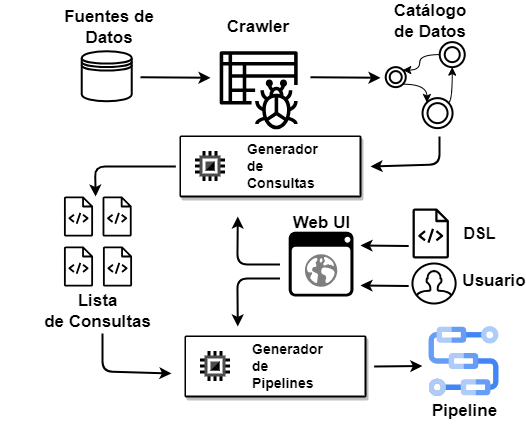
\includegraphics[width=0.60\textwidth]{Graphics/arch.drawio.png}
    \caption{Arquitectura del prototipo de AutoETL}
    \label{fig:arquitectura}
    \end{figure}

AutoETL se concibe como una herramienta para ser utilizada por los desarrolladores de almacenes de datos 
con el objetivo de aliviar la carga de trabajo en la implementaci\'on de los procesos de población de las 
estructuras analíticas. Como se observa en la Figura \ref{fig:arquitectura} los componentes de la aplicaci\'on 
est\'an dispuestos de forma secuencial para representar el flujo de trabajo de la herramienta.

